% ***************************** MAIN FILE **********************************

\documentclass[12pt]{report}           % Art des zu erstellenden Dokuments
% bei zweiseitigem Druck twoside-Option oder book-Klasse verwenden

% ****************************** PREAMBLE **********************************
% **************************** PACKAGE SETUP *******************************
\usepackage[ngerman]{babel}          % Lokalisierung von Typographie, Silbentrennung, etc.
\usepackage{geometry}                % Zum Gestallten der Seiten
\usepackage{ucs}                     % Erweiterte Unterstützung von UTF-8-Kodierung
\usepackage[utf8x]{inputenc}         % Unterstützung von UTF-8 in Eingabe-Dateien
\usepackage[T1]{fontenc}             % Zeichensatzkodierung von LaTeX (Cork-Kodierung)
\usepackage{helvet,courier,mathptmx} % Verwendete Schriftarten

\usepackage{amsmath}                 % Mathematische Infrastruktur für LaTeX der AMS
\usepackage{amsfonts}                % Mathematische Schriftarten
\usepackage{amssymb}                 % Mathematische Symbole
\usepackage{amsthm}                  % Erweiterung der Theorem-Umgebungen

\usepackage{fancyhdr}                % Erweiterte Konfiguration von Kopf/Fußzeile
\usepackage{hyperref}                % Querverweise, Hyperlink, pdf-Konfiguration, etc.
\usepackage[
nonumberlist, %keine Seitenzahlen anzeigen
nopostdot,    %Den Punkt am Ende jeder Beschreibung deaktivieren
acronym,      %ein Abkürzungsverzeichnis erstellen
toc,          %Einträge im Inhaltsverzeichnis
section,      %im Inhaltsverzeichnis auf section-Ebene erscheinen
%numberedsection=autolabel %Zum einfügen in das Appendix
]{glossaries}					     % vor hyperref einbinden, um Verlinkung zu deaktiveren

\usepackage{float}                   % Selbstdefinierte Floating-Umbgebungen
\usepackage{tabularx}                % Tabellen mit einstellbarer Spaltenbreite
\usepackage[labelfont=bf]{caption}   % Anpassen der Abbildungs- und Tabellenbeschriftungen

\usepackage{algpseudocode}           % Algorithmen als Pseudocode (basiert auf algorithmicx)
\usepackage{listings}                % Quellcode-Satz (z.B. mit Syntax-Hervorhebung)

\usepackage{graphicx}                % Erweiterte Unterstützung von Graphiken
\usepackage{textpos}                 % Beliebig platzierte Textboxen
\usepackage{xcolor}                  % TeX-Engine-unabhängige Definition von Farben

\usepackage[numbers]{natbib}         % Weiter Optionen für die Bibliographie

\usepackage{setspace}
\usepackage{ellipsis}	% Korrigiert den Wei�raum um Auslassungspunkte
\usepackage{placeins} 
\usepackage{tikz}

% ****************************** TOP MATTER ***********************************
\renewcommand{\author}{Stefan Kruk}           % Name
\newcommand{\dateOfBirth}{14.08.1992}           % Geburtsdatum
\newcommand{\matrNumber}{7084972}              % Matrikelnummer
\newcommand{\studycourse}{Softwaretechnik (Dual)}           % Studiengang

\newcommand{\supervisor}{Prof. Dr. Johannes Ecke-Schüth} % Betreuer
\newcommand{\institution}{Fachhochschule Dortmund} % Hochschule
\newcommand{\faculty}{Informatik}               % Fachbereich
\newcommand{\toponym}{Dortmund}                 % Ort

\newcommand{\subject}{Projektarbeit}  % Art/Thema der Arbeit
\newcommand{\titel}{Gemeinsamkeiten und Unterschiede von Software-Orientierte-Architektur (SOA) und Microservices} % Titel der Arbeit
%\newcommand{\subtitel}{Zweizeiliger Untertitel\\sofern vorhanden} % Untertitel
\newcommand{\degree}{Bachelor/Master of Art\xspace} % Angestrebter Titel (nur bei Abschlussarbeiten, sonst leer lassen/auskommentieren)

\newcommand{\keywords}{Projektarbeit, SOA, Microservices, Informatik, {FH Dortmund}} % Stichworte (durch Komma getrennt)

% **************************** HYPERREF SETUP *******************************
\definecolor{linkcolor}{rgb}{1,0.5,0}
\hypersetup
{
bookmarks=true,                        % Lesezeichen im PDF erzeugen
bookmarksopen=true,                    % Lesezeichen im PDF sofort anzeigen
backref=true,                          % Rückverweise im Literaturverzeichnis
colorlinks=true,                       % Farbige Verweise
%hidelinks = true,                      % Verweise verbergen (entfernt Farbe und Rahmen)
pdfstartview={FitH},                   % Ansicht des PDFs beim öffnen
pdftitle={\titel},                     % Title des PDFs
pdfauthor={\author , \supervisor},     % Autor des PDFs
pdfsubject={\subject},                 % Thema des PDFs
%pdfcreator={Creator},                 % Erzeuger des Dokuments (Anwendungsprogramm)
%pdfproducer={Producer},               % Ersteller des PDFs (Programm/Bibliothek/Skript)
pdfkeywords={\keywords},               % Stichwörter zum PDF
linkcolor=linkcolor,                   % Farbe von Querverweisen
citecolor=orange,                       % Farbe von Zitaten
filecolor=magenta,                     % Farbe von Verweisen auf Dateien
urlcolor=cyan                          % Farbe von URLs
}
% Weitere Optionen: http://www.tug.org/applications/hyperref/manual.html

% Für Zeichnungen
\usetikzlibrary{% 
    arrows,% 
    calc,% 
    fit,% 
    patterns,% 
    plotmarks,% 
    shapes.geometric,% 
    shapes.misc,% 
    shapes.symbols,% 
    shapes.arrows,% 
    shapes.callouts,% 
    shapes.multipart,% 
    shapes.gates.logic.US,% 
    shapes.gates.logic.IEC,% 
    er,% 
    automata,% 
    backgrounds,% 
    chains,% 
    topaths,% 
    trees,% 
    petri,% 
    mindmap,% 
    matrix,% 
    calendar,% 
    folding,% 
    fadings,% 
    through,% 
    positioning,% 
    scopes,% 
    decorations.fractals,% 
    decorations.shapes,% 
    decorations.text,% 
    decorations.pathmorphing,% 
    decorations.pathreplacing,% 
    decorations.footprints,% 
    decorations.markings,% 
    shadows
} 

% **************************** LISTINGS SETUP *******************************
\definecolor{keywords}{rgb}{0.5 0 0.3}
\definecolor{comments}{rgb}{0.25,0.5,0.37}
\definecolor{lila}{RGB}{112, 6, 147}
\definecolor{kommentgreen}{RGB}{5,132,71}
\definecolor{grey}{RGB}{242,242,242}  
\definecolor{darkgreen}{named}{green}
\definecolor{darkblue}{named}{blue}
\definecolor{lightblue}{RGB} {63,95,191}
\definecolor{darkred}{named}{red}
\definecolor{grau}{named}{gray}
\definecolor{fh_orange}{rgb}{0.953,0.201,0}
\definecolor{fh_grau}{rgb}{0.76,0.75,0.76}

\definecolor{listinggray}{gray}{0.9}
\definecolor{lbcolor}{rgb}{0.9,0.9,0.9}
\lstset{literate=%
    {Ö}{{\"O}}1
    {Ä}{{\"A}}1
    {Ü}{{\"U}}1
    {ß}{{\ss}}1
    {ü}{{\"u}}1
    {ä}{{\"a}}1
    {ö}{{\"o}}1
    {~}{{\textasciitilde}}1
}
\lstset{ %
    backgroundcolor=\color{grey},   % Hintergrundfarbe
    basicstyle=\linespread{0.94}\footnotesize\ttfamily, % Schrifteinstellungen für Quellcode
    breakatwhitespace=false,         % Automatische Zeilenumbrüche nur bei Leer- oder Tabulatorzeichen (Leerraum/whitespaces)
    breaklines=true,                 % Automatische Zeilenumbrüche
    captionpos=b,                    % Beschriftung unten
    commentstyle=\color{comments},   % Schrifteinstellungen für Kommentare
    columns=felxible,                 % Ist notwendig, damit man Quellcode aus den Listings kopieren kann
    %  deletekeywords={...},            % Bestimmte Schlüsselwörter entfernen
    escapeinside={\%*}{*)},          % Defintion von Escape-Sequenzen
    extendedchars=false,                   % Nicht ASCII-Zeichen erlauben
    frame=single,                    % Rahmen um den Quellcode
    keepspaces=true,                 % Einrückungen im Quellcode behalten
    keywordstyle=\bfseries\color{keywords},% Schrifteinstellungen für Schlüsselwörter
    language=java,                   % Programmiersprache des Quellcodes
    %  morekeywords={*,...},            % Zusätzliche Schlüsselwörter
    numbers=left,                    % Zeilennummerierung
    numbersep=5pt,                   % Abstand zwischen Zeilennummerierung und Quellcode
    numberstyle=\color{black}, % Schrifteinstellungen für Zeilennummern
    rulecolor=\color{black},         % if not set, the frame-color may be changed on line-breaks within not-black text (e.g. comments (green here))
    showspaces=false,                % Leerraum-Zeichen anzeigen
    showstringspaces=false,          % Leerzeichen in Zeichenketten anzeigen
    showtabs=false,                  % Tabulatorzeichen in Zeichenketten anzeigen
    stepnumber=1,                    % Schrittweite bei Zeilennummern
    stringstyle=\color{blue},        % Schrifteinstellungen für Zeichenketten
    tabsize=4,                       % Tabulatorbreite (Anzahl Leerzeichen)
    numberbychapter=false            % Nummeriere Quellcode fortlaufend je Kapitel
}

\lstdefinestyle{java}
{
    language=Java,
    keywordstyle=\bfseries\color{lila},  	% underlined bold black keywords 
    identifierstyle=\bfseries\color{blue}, 
    commentstyle=\bfseries\color{kommentgreen}, % white comments 
    stringstyle=\bfseries\color{black},
}

\lstdefinestyle{xml}
{
    language=xml,
    basicstyle=\fontsize{9pt}{9pt}\selectfont\color{kommentgreen},
    keywordstyle=\color{lila},  	% underlined bold black keywords 
    %Hier können bei Bedarf noch weitere Keywords eingetragen werden
    keywords={name, value, version, encoding, id, type, xmlns:xsi, ref, namespace},
    identifierstyle=\color{black},  
    stringstyle=\color{blue},  
    commentstyle=\color{lightblue},
    morecomment=[s]{<!--}{-->},
    rulecolor=\color{black}
}
\renewcommand{\lstlistlistingname}{Quellcode}
\renewcommand{\lstlistingname}{Quellcode}

\AtBeginDocument{\numberwithin{lstlisting}{section}} % Nummeriere Quellcode fortlaufend je Abschnitt

% ************************** HEADER/FOOTER SETUP ****************************
\setlength{\headheight}{15pt}

\renewcommand{\chaptermark}[1]{ \markboth{#1}{} }

\fancyhf{}
\fancyhead[LE]{\thepage \ \ \ \ {\tiny \author, \today}}
\fancyhead[RO]{{\tiny \author, \today} \ \ \ \ \thepage}
\fancyhead[LO,RE]{\textit{\nouppercase{\leftmark}} }
\renewcommand{\headrulewidth}{0pt}

% **************************** GRAPHICX SETUP *********************************
\DeclareGraphicsExtensions{.pdf,.png,.jpg} % bekannte Graphik-Dateiformate (müssen nicht mehr im Dateinamen angegeben werden, also statt "beispiel.png" nur noch "beispiel")
\graphicspath{{./figure/}}   % path to graphics folder, usage {PATH},{ANOTHERPATH}...

% ************************** BIBLIOGRAPHY SETUP ********************************
\bibliographystyle{dinat}    % Literaturverzeichnis nach DIN
%\AtBeginDocument{\nocite{*}}    % Diese Zeile vor der Abgabe der Arbeit entfernen!

% ****************************** MATH SETUP ************************************
\everymath{\displaystyle}    % Erzwinge \displaystyle für Mathematischen-Modus


% ************************* THEOREMS AND PROOF *********************************
\newtheoremstyle{thesis}     % Name des neuen Theorem-Stils
{3pt}                        % Abstand oberhalb des Theorems
{3pt}                        % Abstand unterhalb des Theorems
{\itshape}                   % Schrifteinstellungen innerhalb des Theorems
{}                           % Einrückung der Theorem-Überschrift
{\bfseries}                  % Schrifteinstellungen für die Überschrift des Theorems
{}                           % Satzzeichen zwischen Überschrift und Theorem-Rumpf
{\newline}                   % Abstand hinter der Überschrift
{}                           % Spezifikation der Überschrift
  
\theoremstyle{thesis}        % Verwende neuen Theorem-Stil

\newtheorem{theorem}{Satz}[section] % neue Theorem-Umgebung: theorem (Satz)
\providecommand*{\theoremautorefname}{Satz} % autoref-Name für theorem

\newtheorem{definition}{Definition}[section] % neue Theorem-Umgebung: definition (Definition)
\providecommand*{\definitionautorefname}{Definition} % autoref-Name für definition

\renewcommand{\qedsymbol}{$\blacksquare$} % Schwarzes Quardrat als Symbol für: q. e. d.
\renewenvironment{proof}[1][\proofname]{{\bfseries #1:}~}{\qed} % "Beweise:" in Fettdruck

% *************************** PSEUDOCODE SETUP ********************************
\floatstyle{boxed}                        % Rahmen für pseudocode-Umgebung
\newfloat{pseudocode}{htbp}{lop}[section] % Definieren pseudocode-Umgebung
\floatname{pseudocode}{Pseudocode}        % Beschrifte pseudocode-Umgebung mit "Pseudocode"

\newcommand{\listofpseudocodename}{Pseudocodeverzeichnis}
\newcommand{\listofpseudocode}{\listof{pseudocode}{\listofpseudocodename}}
\providecommand*{\pseudocodeautorefname}{Pseudocode}

% ******************************* PAGE SETUP **********************************
\textheight23cm
\textwidth14cm
\voffset0cm
\topskip0cm
\topmargin-1.2cm
\headheight1.0cm
\headsep1.5cm
\oddsidemargin1.0cm
\evensidemargin1.0cm
\renewcommand{\baselinestretch}{1.4} 
\widowpenalty=300
\clubpenalty=300

% ******************************** MACROS *************************************
\newcommand{\RR}{\mathbf{R}}
\newcommand{\NN}{\mathbf{N}}
\newcommand{\QQ}{\mathbf{Q}}
\newcommand{\ZZ}{\mathbf{Z}}
\newcommand{\CC}{\mathbf{C}}
\newcommand{\SOA}{Service-orientierte Architektur}
\newcommand{\ebay}{eBay}
\newcommand{\secref}[1]{\ref{#1} \nameref{#1}}

%%%%%%%%%%%%%%%%%%%%%%%%%%%%%%%%%%%%%%%%%%%%%%%%%%%%%%%%%%%%%%%%%%%%%%%%%%%%%%%
% ****************************** Glossarie ************************************
%%%%%%%%%%%%%%%%%%%%%%%%%%%%%%%%%%%%%%%%%%%%%%%%%%%%%%%%%%%%%%%%%%%%%%%%%%%%%%%

%Befehle für Glossar
\newglossaryentry{glos:SOA}{
    name=SOA,
    description={SOA steht für Service-orientierte Architektur und ist ein Architekturmuster für Service-orientierte Systeme. SOA ist in dem Bereich der verteilten Systeme einzuordnen und wird eingesetzt, um Dienste von IT-Systemen zu strukturieren und zu nutzen.}
}

\newglossaryentry{glos:Microservice}{
    name=Microservice, 
    description={Microservices sind ein Architekturmuster aus dem Bereich der verteilten Anwendungen, bei dem komplexe Anwendungen in eigenständige Prozessen zerlegt werden. Diese kommunizieren mit Hilfe von sprachunabhängigen Schnittstellen untereinander. Die Prozesse, welche ebenfalls Microservices genannt werden, sind kleine unabhängige Dienste, welche möglichst nur eine Aufgabe erledigen sollen, diese aber dafür besonders gut. Dadurch ist ein modularer Aufbau von Anwendungssoftware möglich.}
}

\newglossaryentry{glos:Services}{
	name=Services,
	description={Services, zu deutsch Dienste, sind IT-Repräsentanten von fachlichen Funktionalitäten. Dabei sollen Services in sich abgeschlossen (autark) sein, damit diese eigenständig genutzt werden können. Damit Services über das Netzwerk genutzt werden können, müssen wohldefinierte Schnittstellen vorhanden sein. Zusätzlich sollte die Granularität von Services grob sein, um die Abhängigkeiten zu anderen Diensten gering zu halten.}
}

%%%%%%%%%%%%%%%%%%%%%%%%%%%%%%%%%%%%%%%%%%%%%%%%%%%%%%%%%%%%%%%%%%%%%%%%%%%%%%%
% ************************** BEGINN OF DOCUMENT *******************************
%%%%%%%%%%%%%%%%%%%%%%%%%%%%%%%%%%%%%%%%%%%%%%%%%%%%%%%%%%%%%%%%%%%%%%%%%%%%%%%
\begin{document}

\begin{titlepage}
%FH LOGO
% 
\includegraphics[width=3.8cm]{content/images/fh_logo_neu_orange_A4}

% *** Subject ***
{\centering {\Huge \bfseries \subject\par}}
% *** Thema ***
\bigskip\bigskip
{\centering Thema:\\[0.3cm] {\textbf {\large\titel} \\[0.3cm] \ifdefined\subtitel \subtitel  \fi \\[0.05cm]}\par}

\bigskip\bigskip
% *** Author Informationen ***
{\centering\bfseries \author\par}
{\centering geboren am \dateOfBirth\par}
{\centering Matr.-Nr.: \matrNumber\par}


\bigskip\bigskip\bigskip
%*** Hochschulinformationen ***
{\centering An der \institution im Fachbereich \faculty erstellte \par}
{\centering \subject\par}
{\centering im Studiengang \studycourse \par}
 \ifdefined\degree
\bigskip
{\centering   
    zur Erlangung des Grades akademischen Grades \degree \par}
\fi
%*** Betreuer Informationen ***
\bigskip\bigskip\bigskip
{\centering \textbf{Betreuer:} \supervisor \par}

%*** Hochschul Logo
\bigskip\bigskip\bigskip
{\centering  
\includegraphics[width=3.8cm]{content/images/fh_logo_neu_orange_A4} \par}
{\centering\bfseries  Fachbereich \faculty\par}

\bigskip\bigskip
{\centering Dortmund, \today\par}

\end{titlepage}


% ***************************** FRONT MATTER **********************************
\setcounter{page}{1}
\pagenumbering{roman}

% *************************** TABLE OF CONTENTS *******************************
% ************************* (Inhaltsverzeichnis) ******************************
% Die Auskommentierte Zeile fügt das Inhaltsverzeichnis zum Inhaltsverzeichnis hinzu. Diese Verhalten kann auch über das Paket tocbibind erreicht werden. Allerdings funktioniert das Paket nicht für das Pseudocodeverzeichnis, aus diesem Grund werden die Einträge "manuell" hinzugefügt.

%\phantomsection\addcontentsline{toc}{chapter}{\numberline{}\contentsname}
{
\baselineskip=15pt % Schriftlinien-Abstand 15 pt (nur beim Inhaltsverzeichnis)
\tableofcontents   % Inhaltsverzeichnis einfügen
}
{
\baselineskip=22pt % Schriftlinien-Abstand 22 pt (bei allen anderen Verzeichnissen)

% **************************** LIST OF FIGURES ********************************
% ************************ (Abbildungsverzeichnis) ****************************
%\clearpage\phantomsection\addcontentsline{toc}{chapter}{\numberline{}\listfigurename}

\listoffigures % Abbildungsverzeichnis einfügen

% **************************** LIST OF TABLES *********************************
%\clearpage\phantomsection\addcontentsline{toc}{chapter}{\numberline{}\listtablename}

%\listoftables % Tabellenverzeichnis einfügen

% ************************** LIST OF PSEUDOCODE *******************************
%\clearpage\phantomsection\addcontentsline{toc}{chapter}{\numberline{}\listofpseudocodename}

%\listofpseudocode % Pseudocodeverzeichnis einfügen

% *************************** LIST OF LISTINGS ********************************
%\clearpage\phantomsection\addcontentsline{toc}{chapter}{\numberline{}\lstlistlistingname}

%\lstlistoflistings % Quellcodeverzeichnis einfügen
}

\chapter*{Überblick}
\section*{Kurzfassung}
In dieser Arbeit werden die Vor- und Nachteile von \SOA\ und Microservices erörtert und anschließend miteinander verglichen werden. Dabei wird explizit auf die Unterschiede und Gemeinsamkeiten der beiden Architekturmodelle eingegangen werden. Für eine bessere Verständlichkeit wird zusätzlich ein bestimmter Prozesskontext mit beiden Modellen implementiert.

\section*{Abstract}
In this Projekt will be the Pro and Cons of service-oriented architecture and Microservices described. After that both architectural models will be compared. In this Process the differences and similarities between these two models will be described. For a better understanding i will implement an application with both architectural models.

%% ******************************* Glossar ************************************
%Alle Glossare ausgeben
%\printglossaries

%Glossar ausgeben
\printglossary[style=altlist,title=Glossar]


%Abkürzungen ausgeben
\deftranslation[to=German]{Acronyms}{Abkürzungsverzeichnis}
\printglossary[type=\acronymtype,style=long]

%Symbole ausgeben
\printglossary[type=symbolslist,style=long]
\newpage

% ***************************** MAIN MATTER ***********************************
\pagestyle{fancy}
\pagenumbering{arabic}

\chapter{Einleitung}
\label{chap:Einleitung}
Die Idee der Aufteilung eines komplexen Softwaresystemes ist nicht neu. Monolithische Systeme bestehen meistens aus mehreren Modulen, welche zusammen zu einer ausführbaren Datei gepackt werden. Es kann jedoch auch möglich, dass Module in eigene Bibliotheken verpackt werden, welche zur Laufzeit geladen werden. Da die Bibliotheken für die korrekte Ausführung der Software notwendig sind, müssen diese mit ausgeliefert werden. Müssen einzelne Programmteile verändert (korrigiert, erweitert, angepasst oder verbessert) werden, muss jede Software, welche diesen Programmteil verwendet neu gebaut und ausgeliefert werden. Dies kann einen erheblichen Aufwand bedeuten, wenn dieser Programmteil in einer großen Anzahl von Software verwendet wird. Daher wurde die Idee entwickelt, Fachlichkeiten in einzelne Dienste (Services) auszulagern und zentral zu verwalten. Das Konzept der Verteilten Anwendungen wurde erstellt.
\\\\
Dieses Konzept wurde nach und nach weiterentwickelt. Zwei Paradigmen, welche diesem Ansatz folgen sind SOA (Service-orientierte Architektur) und Microservices. Beide Paradigmen setzten auf einzelne Services, welche einzelne Fachlichkeiten beinhalten und diese über APIs nach außen anbietet.

\section{Begriffsabgrenzungen}
\label{sec:Begriffsabgrenzungen}

\subsection*{SOA und "`Service-orientierte Architektur"'}
Sowohl SOA als auch Microservices zählen zu dem Paradigma der "`Service-orientierten Architekturen"'.

Die Abkürzung SOA wird hier sowohl für das Paradigma "`Service-orientierte Architektur"' verwendet, wie auch für die spezielle Herangehensweise.

Um die beiden Thematiken in dieser Arbeit abzugrenzen wird der Begriff "`SOA"' für die Herangehensweise verwendet und die ausgeschriebene Variante zur Kennzeichnung des allgemeinen Paradigmas.

\section{Zielsetzung und Aufgabenstellung}
\label{sec:ZielsetzungUndAufgabenstellung}
Ziel dieser Projektarbeit ist es, die Unterschiede und Gemeinsamkeiten von SOA und Microservices zu beleuchten. Es werden sowohl die Einsatzmöglichkeiten, als auch die nötigen Architekturen und Schnittstellen, des jeweiligen Paradigmas, ermittelt. Außerdem werden die Vor- und Nachteile des jeweiligen Paradigmas, bezüglich der Prozessisolierung, Skalierung, Deployment, Wartbarkeit (Korrigierbarkeit, Erweiterbarkeit, Anpassbarkeit, Verbesserung), Entwicklung/Testbarkeit und der Bindung an Technologiestacks herausgearbeitet. 

\section{Vorgehensweise}
\label{sec:Vorgehensweise}
Zu beginn wird eine Problemanalyse von monolithischen Systemen durchgeführt. Danach werden die allgemeinen Grundlagen für die Verwendung von Verteilten Systemen und die damit verbundenen Probleme erläutert. In diesem Zusammenhang werden die Unterschiede zu monolithischen Systemen herausgearbeitet und der Begriff "`Service"' genauer Definiert. Auf dieser Basis werden die Paradigmen SOA und Microservices vorgestellt und genauer beleuchtet.
\\\\
Darauf aufbauend werden die Einsatzmöglichkeiten der jeweiligen Paradigmen analysiert und die dafür nötigen Architekturen und Schnittstellen herausgearbeitet. Insbesondere soll ermittelt werden, welche Plattformen und Voraussetzungen für den Einsatz der jeweiligen Paradigmen notwendig sind. Außerdem werden die Vor- und Nachteile der Paradigmen, hinsichtlich der Prozessisolierung, Skalierung, Deployment, Wartbarkeit (insbesondere der Korrigierbarkeit, Erweiterbarkeit, Anpassbarkeit, Verbesserung), Entwicklung/Testbarkeit und der Bindung an Technologiestacks herausgearbeitet und mit einander verglichen.
\\\\
Abschließend wird ein Fazit aus den gewonnen Erkenntnissen gezogen und ein Ausblick auf weiterführende Arbeiten gegeben.

\chapter{Problemanalyse von Monolithischen Systemen/Anwendungen}
\label{chap:ProblemanalyseMonolithischeSysteme}
In der klassischen Softwareentwicklung sind monolithische Anwendungen oft die Grundlage für komplexe Systeme. Dabei besitzt die Anwendung alle nötigen Ressourcen und Eigenschaften, um eine bestimmte Aufgabe zu erfüllen. Dies fängt an bei der Datenverwaltung, wie zum Beispiel der Persistierung und dem Laden von Daten. Dies kann beispielsweise durch eine Datenbankschnittstelle umgesetzt werden. Dabei wird jedoch meistens nur eine einzelnes Datenbanksystem unterstützt. Neben der Datenverwaltung gehören noch weitere Aufgaben zu einer Anwendung, wie zum Beispiel das Durchführen von verschiedenen Berechnungen auf Grundlage der vorhandenen Daten. Damit ein Benutzer eine Anwendung benutzen kann, muss zudem eine Benutzerinterface vorhanden sein. Dies kann zum Beispiel durch eine Internetseite  oder durch eine native Desktop Darstellung geschehen.

\section{Herausforderungen bei der Verwendung von monolithischen Systemen}
\label{sec:HerausforderungenMonolithisch}
Zu Beginn der Entwicklung stellt das Erstellen einer Anwendung, auf Basis eines Pflichtenheftes keine große Herausforderung dar. Es können die Anforderungen an das neue System analysiert werden und darauf aufbauend eine Programmiersprache und die interne Architektur gewählt werden.
\\\\
Werden hingegeben, bei einer bestehenden Anwendung, neue Anforderungen gestellt, ist man zunächst einmal an den zuvor gewählten Technologie-Stacks gebunden. Das Korrigieren von Fehlern ist relativ einfach, im Vergleich zur Anpassbarkeit und Erweiterbarkeit des Systems. Je nach Größe der Anwendung, kann dadurch die Umsetzung der neuen Anforderungen problematisch werden, sofern diese nicht mit den bestehenden internen Architekturen vereinbar sind. In diesem Fall kann die Anforderung dazu führen, dass die Anwendung umgeschrieben oder im schlimmsten Falle neu geschrieben werden muss.
\\\\
Ein weiteres Problem besteht in der parallelen Weiterentwicklung.
\begin{quotation}
    \frqq Es gibt Teams, die an verschiedenen neuen Features arbeiten. Aber die parallele Arbeit ist kompliziert: Die Struktur der Software ist dafür zu schlecht. Die einzelnen Module sind zu schlecht separiert und haben zu viele Abhängigkeiten untereinander. \flqq\ \cite[S. 16]{EWolff2016:Microservices}
\end{quotation}
Ohne eine Versionsverwaltung ist das parallele Arbeiten nicht möglich, da ansonsten die Gefahr zu groß ist, Programmteile von anderen Teams, ungewollt zu überschreiben. Ein weiteres Problem besteht bei der Durchführung von Integrationstests.

\begin{quotation}
    \frqq Wenn der Deployment-Monolith durch einen Integrationstest läuft, dürfen in dem Test nur die Änderungen eines Teams enthalten sein. Es gab Versuche, mehrere Änderungen auf einmal zu testen. Dann war bei einem Fehler nicht klar, woher das Problem kam, und es gab lange und komplexe  Fehleranalysen.\flqq\ \cite[S. 16]{EWolff2016:Microservices}
\end{quotation}
Dadurch entsteht ein Flaschenhals, da andere Teams warten müssen, bis die Integrationstests erfolgreich durchlaufen wurden.


\subsection{Skalierung}
\label{subsec:SkalierungMonolithisch}
Skalierung ist ein wichtiges Thema von Webanwendungen. Greifen viele Benutzer auf eine Anwendung zu, so kann es dazu führen, dass dies das System überlastet und alle Benutzer länger auf die Antwort des Systems warten müssen. Um dies zu verhindern, müssen Anwendungen skaliert werden.

\begin{quotation}
    \frqq Skalierbarkeit bedeutet, dass ein System mehr Last bearbeiten kann, wenn es mehr Ressourcen bekommt.\flqq\ \cite[S. 150]{EWolff2016:Microservices}
\end{quotation}

Es gibt nach \cite[S. 150]{EWolff2016:Microservices} zwei verschiedene Arten der Skalierbarkeit:
\begin{itemize}
    \item \textit{Horizontale Skalierbarkeit} bedeutet, dass mehr Ressourcen zur Verfügung stehen, die jeweils einen Teil der Last bearbeiten, die Anzahl der Ressourcen steigt also.
    \item \textit{Vertikale Skalierbarkeit} bedeutet, dass leistungsfähigere Ressourcen genutzt werden, um mehr Last handzuhaben. Eine einzelne Ressource wird also mehr Last abarbeiten. Die Anzahl der Ressourcen bleibt konstant.
\end{itemize}

Beide Arten der Skalierbarkeit haben ihre Vor- und Nachteile. Welche Art benutzt wird, muss im individuell entschieden werden, jedoch ist die vertikale Skalierung bei Monolithen, meistens deutlich einfacher, als die horizontale Skalierung.

\chapter[Grundlagen von Service-orientierten Systemen]{Allgemeine Grundlagen zur Verwendung von Service-orientierten Systemen}
\label{chap:Grundlagen}
Ein Service-orientiertes System, ist ein Architekturmuster, bei dem einzelne Dienste (Services) ein IT-System bilden. Es liegt dem Bereich der verteilten Systemen zur Grunde und dient oft zur Strukturierung von komplexen Systemen.
\\\\
Anstatt eine einzige große Anwendung ein zu setzten, setzt man auf viele kleine, verteilte, autarke Anwendungen, welche als Dienste bezeichnet werden. Diese bieten nach außen entsprechende Schnittstellen an, um den jeweiligen Dienst nutzen zu können. Dabei ist dieses Architekturmuster eine weitere Form der Modularisierung von Softwaresystemen, da einzelne Komponenten (Fachlichkeiten) durch eigenständige Anwendungen abgebildet werden.

\section{Was ist ein Service?}
\label{sec:WasIstEinService?}
Ein Service ist in einem "`Service-orientiertem System"' eine Fachlichkeit eines gesamt Systems. Es wird versucht autarke Services zu erstellen, welche unabhängig von anderen Diensten verwaltet und verwendet werden können.. Die Größe von Diensten ist dabei jedoch nicht festgelegt und kann je nach Paradigma bzw. Definition und Unternehmen variieren.

\section{Verteilte Systeme}
\label{sec:VerteilteAnwendungen}
Damit Service-orientierte Architekturen verstanden werden können, müssen zunächst verteilte Systeme verstanden werden. \textit{Andrew S. Tanenbaum} definiert ein verteiltes System wie folgt:
\begin{quotation}
    \frqq Ein verteiltes System ist eine Ansammlung unabhängiger Computer, die den Benutzer wie ein einzelnes kohärentes System erscheinen.\flqq\cite[S. 19]{tanenbaum:VerteilteSysteme}
\end{quotation}
Im Falle von Service-orientierten Architekturen wird das System auf mehrere eigenständige Computer bzw. Anwendungen aufgeteilt. Ein Vorteil von verteilten Systemen ist, dass sie Zum einen sehr dynamisch und schnell anpassbar sind, zum Anderen jedoch auch die Komplexität von Software in einzelne Teile zerbricht, wodurch eine entfernte Präsentation möglich ist.
Jedoch entstehen dadurch Probleme, welche in monolithischen Systemen/Anwendungen nicht vorhanden sind.
\\\\
Eines der wichtigsten und größten Probleme besteht dabei in der Kommunikation. Zum Einen muss diese gewährleistet werden, zum Anderen jedoch auch in angemessener Zeit erfolgen. Dabei muss ebenfalls darauf geachtet werden, dass Nachrichten erfolgreich zugestellt werden, selbst wenn einzelne Dienste temporär nicht erreichbar sind.
\\\\
Ein weiteres Problem besteht darin, zu erkennen wann ein Dienst ausgefallen ist. Meistens erkennt man dies nur dadurch, dass ein Teilsystem nicht funktioniert. Das ausgefallene System zu identifizieren stellt, wenn keine entsprechenden Vorkehrungen getroffen wurden, eine nicht zu unterschätzende Problematik da. Zudem kann eine lange Zeit vergehen, bis das Unternehmen merkt, dass ein System ausgefallen ist. 

\subsection{Domain-Driven Design und Bounded Context}
\label{sec:boundedContext}
Domain-Driven Design (DDD) beschreibt dabei die Herangehensweise zur Modellierung von komplexer Software. Dabei ist die Modellierung maßgeblich an die umzusetzende Fachlichkeit gebunden und wird durch diese beeinflusst. Das Ziel jeglicher Software ist es, eine bestimmte Anwendungsdomäne zu unterstützen. Damit dies erfolgreich geschieht, muss Software harmonisch und in höchster Form interoperabel zur Anwendungsdomäne sein. Domain-Driven Design soll genau dies gewährleisten.
\\\\
Arbeitet man mit Service-Orientierten Architekturen, versucht man fachliche Komponenten, welche zu einem bestimmten Kontext gehören, möglichst nahe beieinander zu halten. Man spricht hierbei von \textit{Bounded Context}. 
\begin{quotation}
    \frqq Bounded Context ist ein zentrales Muster in Domain-Driven Design.[..] DDD arbeitet mit großen Modellen, indem es diese in kleine verschiedene zusammengehörige Kontexte unterteilt und auf ihre Wechselwirkung unterteilt.\flqq \cite{mfowler:BoundedContext}
\end{quotation}

\begin{figure}[htb]
    \centering 
    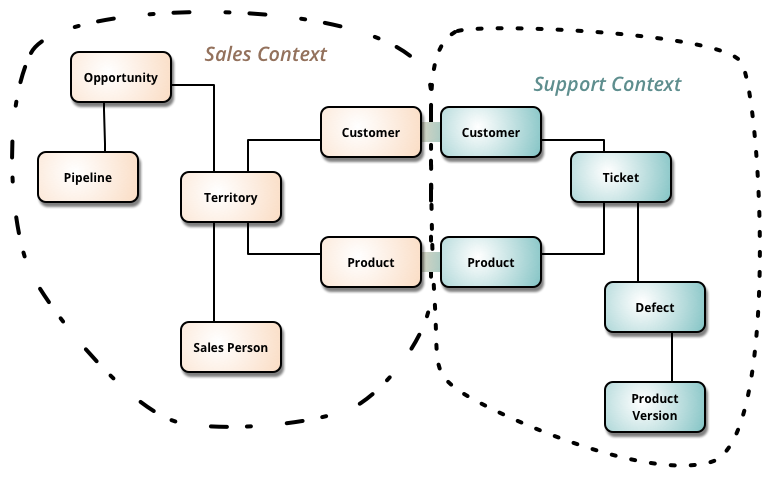
\includegraphics[width=\linewidth]{content/images/BoundedContext}\
    \quelle\url{http://martinfowler.com/bliki/BoundedContext.html}
    \caption[Bounded Context]{Bounded Context\\}
    \label{fig:BoundedContext}  
\end{figure} 
In dieser Grafik wird noch einmal der Begriff Bounded Context genauer verdeutlicht. Es existieren zwei eigenständige Prozesse. Auf der linken Seite der Sales Kontext und auf der rechten Seite der Support Kontext. Jeder Kontext besitzt verschiedene Services, welche benötigt werden um den Prozess durchführen zu können. Lediglich zwischen den \textit{Customer} und \textit{Product} Services besteht eine Verbindung der beiden Prozesse.

\subsection{Das Gesetzt von Conway}
\label{subsec:conway}
Spricht man von "`Service-orientierten Architekturen"', sollte das \glqq Gesetzt von Conway\grqq\ nicht fehlen, da es Prinzipien beschreibt, nach denen eine Unternehmens-Architektur entworfen wird.
\\\\
Melvin Conway ist ein amerikanischer Informatiker und formulierte seine Beobachtungen bezüglich der Kommunikationsstrukturen und Organisationen innerhalb eines Unternehmens. Seine Beobachtung, auch \glqq Gesetzt von Conway\grqq\ genannt lautet wie folgt:
\begin{center}
    \textit{Organisationen, die Systeme designen, können nur solche Designs entwerfen, welche die Kommunikationsstruktur dieser Organisationen abbilden.}
\end{center}

Conway möchte damit ausdrücken, dass die internen Kommunikationswege wichtig bei der Planung der Architektur ist. Jedes Team innerhalb einer Organisation trägt zu der Entwicklung der Architektur bei. Wird eine Schnittstelle zwischen zwei Teams benötigt, so müssen diese Teams auch kommunizieren können. Dabei müssen Kommunikationswege nicht immer offiziell sein. Oft gibt es informelle Kommunikationsstrukturen, die ebenfalls in diesem Kontext betrachtet werden können.
\\\\
Service-orientierte Systeme arbeiten nach dem gleichen Prinzip. Dienste in diesen Systemen sind eigenständig und müssen, damit daraus eine funktionierende Anwendung bzw. System wird, unter einander problemlos kommunizieren können.

\section{Kommunikation: Orchestration vs Choreographie}
\label{sec:OrchestrationVsChoregraphie}

\subsection*{Orchestration}
\label{subsec:orchestration}
Bei der Orchestration handelt es sich um eine Komposition von Services. Ein Geschäftsprozess wird zwar mit Hilfe von mehreren Services abgebildet, jedoch ist nur ein Service dafür zuständig den Geschäftsprozess durchzuführen.
\newpage
\begin{figure}[htb]
    \centering 
    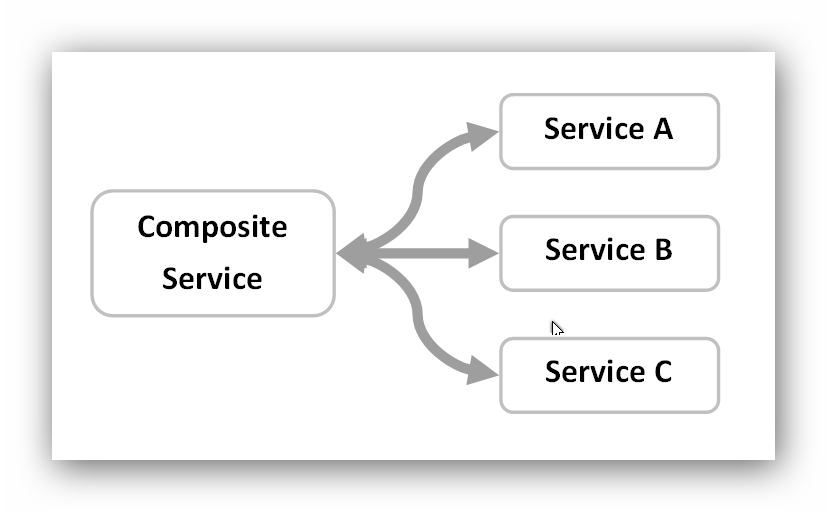
\includegraphics[width=\linewidth]{content/images/ServiceOrchestration}\
    \caption[Orchestration]{Orchestration}
    \label{fig:ServiceOrchestration}  
\end{figure}

Wie die Abbildung \ref{fig:ServiceOrchestration} zeigt besteht bei der Orchestration \textbf{\underline{keine}} Verbindung zwischen:
\begin{itemize}
    \item A \& B
    \item A \& C
    \item B \& C
\end{itemize}
Nur der "`Composite Service"' nutzt die anderen Services, um den Geschäftsprozess abzubilden.

\subsection*{Choreographie}
\label{subsec:choreographie}
Anders als bei der Orchestration können Services bei der Choreographie beliebig untereinander kommunizieren. Das ist sinnvoll, wenn verschiedene Dienste, sich untereinander über Änderungen oder andere Aktionen informieren müssen.
\newpage
\begin{figure}[htb]
    \centering 
    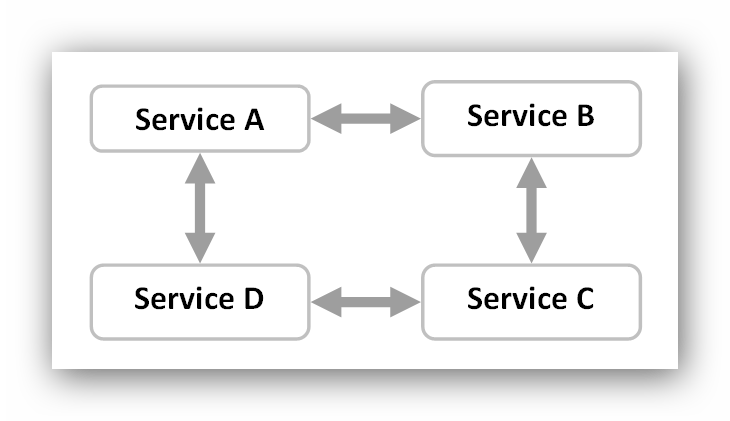
\includegraphics[width=\linewidth]{content/images/ServiceChoreography}\
    \caption[Choreographie]{Choreographie}
    \label{fig:ServiceChoreography}  
\end{figure}
So ist, wie in Abbildung \ref{fig:ServiceChoreography} zu erkennen, eine beliebige Kommunikation zwischen den einzelnen Diensten möglich.

\section{Abgrenzung von monolithischen Systemen}
\label{sec:AbgrenzungVonMonolithischenSystemen}
Im Vergleich zu monolithischen Systemen, muss bei dem Einsatz von Service-orientierten Systemen einiges beachtet werden. So ist die Kommunikation ein wichtiger Faktor. Man muss sich nicht nur zwischen einer der beiden zuvor genannten Kommunikationsformen, Choreographie oder Orchestrierung, entscheiden, es muss zudem sichergestellt werden, dass Nachrichten zugestellt werden.
\\\\
Während bei einem monolithischen System alle Abhängigkeiten innerhalb der Anwendung zu finden sind, besteht die Anwendung in einem Service-orientieren System aus mehreren Diensten, welche untereinander kommunizieren. Jeder Dienst bildet dabei einen gewissen Context ab (siehe \nameref{sec:boundedContext}). Zudem ist es dadurch möglich, dass jeder Dienst eine eigene Datenbank hat, wodurch verschiedene Datenbanksysteme (SQL und NoSQL) eingesetzt werden können. In der nachfolgenden Abbildung ist einem Monolithen, ein Microservice System entgegen gesetzt.
\begin{figure}[htb]
    \centering 
    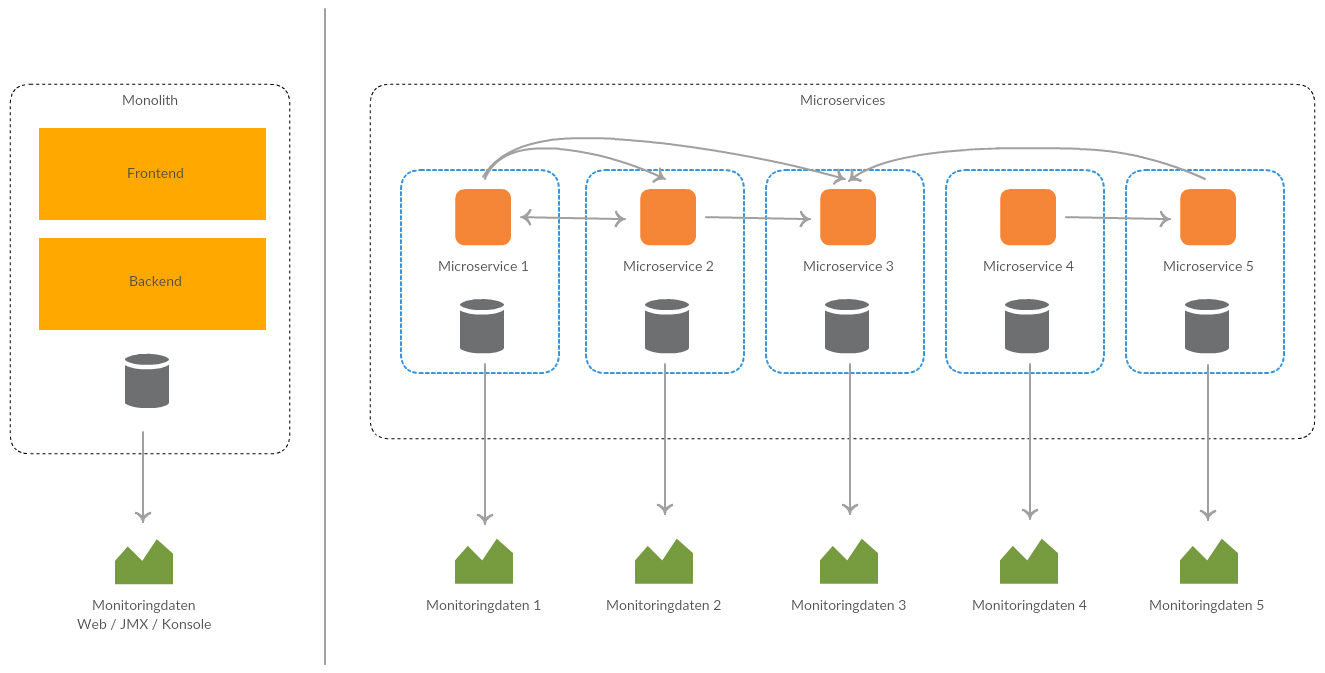
\includegraphics[width=\linewidth]{content/images/fichtner_microservices_1}\
    \quelle\url{https://jaxenter.de/wp-content/uploads/2016/10/fichtner_microservices_1.jpg}
    \caption{Monolithisches vs Service-orientiertes System}
    \label{fig:BoundedContext}  
\end{figure}
Zusätzlich zu den oben genannten unterschieden, sieht man in der Abbildung außerdem ein Monitoring-System. Während bei einem Monolithen, nur ein Monitoring-System benötigt wird, muss bei einem Service-orientiertem System, jeder Service ein Monitoring-System besitzen. Bei großen Systemen, müssen zudem die Monitoring-Informationen gebündelt werden und zentral einsehbar sein.

% ***************************** BIBLIOGRAPHY **********************************
\baselineskip=14pt
\addcontentsline{toc}{chapter}{\protect\numberline{}\bibname}
\bibliography{bib/thesis}

% ******************************* APPENDIX ************************************
\appendix
\baselineskip=18pt
\chapter{Diagramme und Tabelle}
\label{chap:anhang_a}


% ***************************** BACK MATTER ***********************************
\pagestyle{empty}

\addcontentsline{toc}{chapter}{\protect\numberline{}Eidesstattliche Erklärung}
\chapter*{}
\vspace*{0.5cm}
\noindent
{\bf Eidesstattliche Erklärung} \\
Ich versichere an Eides statt, dass ich die vorliegende Arbeit selbständig
angefertigt und mich keiner fremden Hilfe bedient, sowie keine anderen als die
angegebenen Quellen und Hilfsmittel benutzt habe. Alle Stellen, die wörtlich
oder sinngemäß veröffentlichten oder nicht veröffentlichten Schriften und
anderen Quellen entnommen sind, habe ich als solche kenntlich gemacht. Diese
Arbeit hat in gleicher oder ähnlicher Form noch keiner Prüfungsbehörde
vorgelegen. 

\vspace{1cm}
\toponym, den \today \hfill \author


\vspace*{3cm}
\noindent
{\bf Erklärung} \\
Mir ist bekannt, dass nach § 156 StGB bzw. § 163 StGB eine falsche
Versicherung an Eides Statt bzw. eine fahrlässige falsche Versicherung an
Eides Statt mit Freiheitsstrafe bis zu drei Jahren bzw. bis zu einem Jahr oder
mit Geldstrafe bestraft werden kann. 

\vspace{1cm}
\toponym, den \today \hfill \author


%%%%%%%%%%%%%%%%%%%%%% NICHT IN ARBEIT ÜBERNEHMEN!!! %%%%%%%%%%%%%%%%%%%%%%%%%%
%\newpage
%\noindent
%\vspace*{6cm}
%\begin{center}
%{\bf Spezielle Erklärung vor Beginn der Bachelor-Thesis/Master-Thesis}
%\end{center}
%Hiermit erkläre ich, dass ich die vorausgehenden Seiten, die man sich unter 
%\\[0.2cm]
%{\scriptsize \bf \hspace*{0.3cm}ftp://gatekeeper.informatik.fh-dortmund.de/pub/professors/lenze/thesis/thesis.pdf} \\[0.2cm]
%ansehen kann, mit den Erläuterungen zum Aufbau, zum Umfang und zum Inhalt einer
%Bachelor-/Master-Arbeit sorgfältig 
%gelesen und verstanden habe. Insbesondere ist mir klar, was man unter
%wissenschaftlichem Arbeiten versteht und dass korrektes Zitieren ein
%wesentliches Element in diesem Zusammenhang ist. Alle Fragen, die es in diesem
%Kontext noch gab, habe ich inzwischen mit Herrn Lenze geklärt, und es bestehen
%keine Unklarheiten mehr. Über die besondere Problematik von Plagiaten und den
%Kriterien, die ein Vorliegen anzeigen, bin ich ebenfalls genau unterrichtet.
%
%\vspace{1.5cm}
%\toponym, den \\
%\ \ \  \ \ \hspace*{8cm} {\tiny Unterschrift!} \\
%
%\vfill

\end{document}
